\documentclass[11pt]{article}
\usepackage[margin=1.1in]{geometry}
\usepackage{amsmath,amssymb}
\usepackage{booktabs}
\usepackage{graphicx}
\usepackage{microtype}
\usepackage[hidelinks]{hyperref}
\usepackage[numbers,sort&compress]{natbib}
\usepackage{xcolor}

% Working note: citations drafted from working notes — verify every entry
% against primaries before submission.

\newcommand{\lostfact}{lost-fact incident rate}
\newcommand{\evfrac}[1]{$f{=}#1$}

\title{Routable and Unroutable Loss: Certifying Compressed LLM Memory
Along Pointwise and Aggregative Axes}

\author{%
  \textit{Draft v0.3 --- 2026-07-08 --- eviction+synthesis regimes; numbers
  frozen per ABLATION and M3.5 addenda}\\
  \textit{Artifacts: \texttt{memsub-artifacts:/\{gate-eval,
  compactor-certification\}/*.json}}}
\date{}

\begin{document}
\maketitle

\begin{abstract}
``Long context'' conflates a serving problem---fitting the tokens---with two
capability problems that separate the moment full attention becomes
unaffordable: \emph{pointwise} recall of exact, low-redundancy facts, and
\emph{aggregative} understanding of distributed, redundant content. We
introduce a certification protocol that scores the two axes separately,
forbids blending them, and requires every configuration to ship with its
own noise-floor and baseline rows --- then apply it to BOTH major families
of KV compression on Qwen3-4B over a ${\sim}1$B-token, four-domain corpus
of 98{,}355 counterfactually filtered questions. Under untrained eviction
the axes split almost completely: next-token KL stays near
$3{\times}10^{-2}$ while $0.45$--$0.55$ of facts in evicted spans are
silently lost (noise floor $0.000$). A decoupled sufficiency gate ---
a ${\approx}\$140$ calibrated probe over frozen embeddings (test ECE
$0.017$--$0.023$) --- cuts that loss by $72\%$ ($0.52 \rightarrow 0.146$
[bootstrap CI $0.136$--$0.156$]) at $16.8\%$ expansion (oracle $19.4\%$),
strictly dominating query-type routing. Under a trained Still-class
synthesis compactor, certified with the identical protocol at matched
retained budget, the picture inverts: the compactor \emph{halves} untreated
needle loss ($0.583 \rightarrow 0.271$ on the certification protocol) but
degrades the aggregation axis past eviction and collapses at recurrence
depth 4 --- and the refreshed gate's marginal value drops to $22.5\%$
($0.189 \rightarrow 0.146$ on the labeling protocol) at $86\%$ of the
oracle budget. This is the paper's central finding, an asymmetry we call
\textbf{routable vs.\ unroutable loss}: eviction produces large loss that
is highly routable (its cause is mechanical --- overlap with the eviction
window --- so a gate needs no content understanding, evicted-only AUC
$0.62$ carried almost entirely by mechanics features), while synthesis
produces smaller loss that is largely unroutable (its cause is what the
compactor failed to keep, demanding content signal that neither mechanics
nor frozen embeddings supply; AUC $0.55$, decomposition inverted).
Compressor choice therefore determines gate-ability, and a memory system
must report not just how much it loses but how much of that loss its
router can recover. Supporting findings: a multi-hop cost overhang
($2.2$--$2.3\times$ oracle expansion, bounded by the same content-signal
gap), calibration non-transfer across domains (repaired by a shipped
per-domain Platt procedure), and depth-certification machinery that
refuses to stack compactions past the certified recurrence depth.
\end{abstract}

\section{Introduction}

Benchmarks, methods papers, and product claims routinely report a single
``long-context'' score. This paper's starting point is that no such single
number can be coherent once the context no longer fits in exact form. A
needle-class query---an identifier, a figure, a verbatim clause---concentrates
its answer in exact bytes with near-zero redundancy against the surrounding
context; any lossy transform destroys it at a rate proportional to the
compression ratio, and the optimal mechanism for it is selection, indexing,
and exact lookup. An integration-class query---summarization, theme
tracking, most document reasoning---lives on distributed, redundant
information; it is compression-tolerant and often mildly
compression-benefited. The two are not merely different but antagonistic:
compression bought for the aggregative workload is paid for in pointwise
fidelity, and exact retention kept for needles is memory that compression
was meant to free.

If the antagonism is real, three things follow. Evaluation must report the
two axes separately, because a blended score lets a method win the aggregate
while being needle-dead. Compressed-memory systems need a \emph{routed
two-path architecture}---a lossy tier for aggregation and a lossless raw
path for pointwise traffic---rather than a single representation with a
quality knob. And the router itself becomes the critical learned component:
a calibrated, per-query estimate of whether the compressed representation
suffices.

We contribute, in order:
\textbf{(i)} a two-axis certification protocol for compressed LLM memory,
with counterfactually filtered probes such that a correct answer proves the
information flowed through the (compressed) cache;
\textbf{(ii)} a measurement at ${\sim}1$B-token scale across four document
domains showing the axes split under untrained KV eviction---aggregative
fidelity essentially intact, pointwise fidelity collapsing, the gap widening
with eviction fraction;
\textbf{(iii)} a decoupled sufficiency gate---trained entirely outside the
frozen base model for ${\approx}\$140$---that restores the pointwise axis at
a fifth of the always-expand cost, with calibration good enough to expose as
a probability, together with an ablation showing its signal is
predominantly eviction mechanics rather than content;
\textbf{(iv)} two phenomena we believe are documented here for the first
time: the multi-hop \emph{cost overhang}, where a well-calibrated single-hop
gate protects multi-hop correctness only by systematically over-expanding,
and \emph{calibration non-transfer}, where discrimination generalizes across
domains but calibrated probabilities do not;
\textbf{(v)} the headline result, from a small-scale but fully-certified
comparison of trained amortized synthesis against untrained eviction under
the identical protocol: the \emph{routable/unroutable loss} asymmetry.
Eviction deletes needles that synthesis partially preserves, and synthesis
degrades the aggregation axis that eviction leaves nearly intact at
matched budget---but the deeper difference is what a router can do about
the residue. Eviction's loss is mechanically caused and therefore highly
routable (a gate removes $72\%$ of it without any content understanding);
synthesis's loss is content-dependent and largely unroutable with the
signals available to a decoupled gate ($22.5\%$ marginal reduction).
Compressor choice determines gate-ability, so a compressed-memory system
must be certified on loss \emph{and} on the routability of that loss.

\section{Related work}

\paragraph{KV-cache reduction.} Per-context selection scores tokens at
inference and evicts the rest (H2O~\citep{zhang2023h2o},
SnapKV~\citep{li2024snapkv}, StreamingLLM~\citep{xiao2024streamingllm});
amortized selection learns the scorer (KV-Distill~\citep{kvdistill2025});
per-context and amortized synthesis write new compact entries rather than
keeping original rows (Still~\citep{oneill2026still}); architecture-level
lines bake reduction into the model (MLA~\citep{deepseekv2}, native sparse
attention~\citep{yuan2025nsa}). Our work is orthogonal to the choice of
compressor: we certify compressors along two axes and supply the decision
layer their lossiness requires. Notably, the strongest published synthesis
results themselves show the axis split we formalize---near-full aggregative
utility with needle-retrieval collapse---which we take as independent
evidence for the two-workload framing.

\paragraph{Selective prediction and abstention.} The gate is a
selective-prediction head~\citep{geifman2017selective} over an external
memory: it estimates, per query, whether the model's conditioning state
supports the answer. It relates to answerability and abstention heads in
retrieval-augmented settings, with two differences: the label is
\emph{counterfactual} (answers under compressed vs.\ raw conditioning are
compared, rather than correctness being judged in isolation), and the head
is trained fully decoupled from the backbone, using the backbone only
offline as a teacher. Calibration machinery follows \citet{guo2017calibration}
and \citet{platt1999}.

\paragraph{Memory-augmented agents.} OS-style memory hierarchies
(MemGPT-class~\citep{packer2023memgpt}) page text in and out of context but
do not certify fidelity or route by workload; our protocol and gate are
directly applicable to such systems. Blended long-context suites such as
RULER~\citep{hsieh2024ruler} are exactly the evaluations our protocol
unbundles.

\section{Two axes and a certification protocol}
\label{sec:protocol}

\paragraph{Definitions.} Fix a base model $f$, a compression policy $C$, and
a corpus of (context, question, answer) items where each question is
generated from a specific source span. An item is \emph{counterfactually
valid} if $f$ answers it correctly with the context and incorrectly without
it---so a correct answer under compression proves the information traversed
the compressed cache. The \textbf{aggregation axis} is measured over
integrative behavior: next-token KL between $f$ conditioned on the full
cache and $f$ conditioned on $C(\text{cache})$, plus answer-accuracy deltas
on items whose source spans survive compression. The \textbf{pointwise
axis} is the \emph{\lostfact}: among counterfactually valid items whose
source span was compressed away, the fraction answered incorrectly
\emph{without} any expansion mechanism---the silent-failure rate.

\paragraph{Protocol.} A configuration is certified per axis, never as a
blend; the noise floor is established by running the identical probe battery
at zero compression; and a configuration certified only on the aggregation
axis may ship only behind an active, calibrated expansion gate for pointwise
traffic. The last clause converts the antagonism from an observation into a
deployment rule. Every report object embeds an evaluation-protocol record:
the exact item partition entering each axis, the contents of the compacted
context during probing (surviving KV only; no summary text), confirmation
that expansion was disabled, and the scoring rule (argmax over answer-letter
logits, greedy---format failures are structurally impossible).

\section{The eviction regime I: the axes split at 1B-token scale}
\label{sec:split}

\paragraph{Setup.} Base model Qwen3-4B-Instruct-2507 (bf16, greedy, pinned
runtime fingerprint). Corpus: 40{,}000 long documents across financial
filings (238M tokens), literature (416M), case law (119M), and source code
(154M); 98{,}355 extractive multiple-choice items generated by the base
model from random ${\sim}1$k-token sub-chunks, teacher-verified answerable
with context and discarded if answerable without ($98.4\%$ of the 100k
target; code has the lowest filter survival). Equivalence is answer-letter
exact match; a manual audit of the complete pointwise-failure population
(14 unique items) found $0\%$ format noise, ${\approx}80\%$ genuine
forgetting, and $2$--$3$ flawed items. Compression policy:
evict-oldest-non-sink at fractions $0.25$ and $0.40$, with the first four
positions pinned as attention sinks~\citep{xiao2024streamingllm}. Contexts
are 4096-token per-item prefills with item placement randomized by hash,
giving natural exposure to eviction.

\paragraph{Result.} The zero-eviction control gives a lost-fact noise floor
of exactly $0.000$ (conditioned on prior-correct probes; the raw metric
carries a $0.167$ never-knew floor, which is why all headline rates below
condition on prior-correct). Under eviction the aggregation axis barely
moves---mean KL $0.0303$ (\evfrac{0.25}) and $0.0339$ (\evfrac{0.40})
against the full-context teacher, answer deltas on surviving-span items
${\approx}0$---while the pointwise axis collapses: $\mathbf{0.453}$
(\evfrac{0.25}, $n{=}1{,}606$) and $\mathbf{0.551}$ (\evfrac{0.40},
$n{=}3{,}493$) of facts in evicted spans are silently lost. A
matched-random control (same token count evicted uniformly rather than
contiguously) inverts the damage profile---$4\times$ less pointwise loss at
$3\times$ the aggregation KL---showing that recency-structured policies
concentrate pointwise damage exactly where aggregate metrics cannot see it.
One artifact, two workloads, opposite outcomes.

\emph{(Protocol note: an earlier certification pass under packed multi-item
contexts with needle-anchored eviction gave $0.708/0.808$ raw; the canonical
numbers above are re-stated under the per-item randomized-placement protocol
used throughout this paper, with the reconciliation in
Appendix~\ref{app:reconciliation}.)}

\section{The eviction regime II: a decoupled sufficiency gate}

\subsection{Labels, model, calibration}

For each of the 98{,}355 items and each eviction fraction we produce a
counterfactual sufficiency label: $y=1$ iff the answer under the compacted
cache differs from the answer under the raw span (196{,}710 rows; items
whose source span survived eviction enter as natural $y{=}0$ rows). Splits
are grouped by source document, domain-stratified, with an additional
leave-one-domain-out rotation. The gate is a dual encoder over frozen
Qwen3-Embedding-0.6B---the same embedding model that produces the memory
blocks' retrieval shadows---with a 256-d normalized projection interaction,
a small feature head (eviction fraction, query--block overlap, evicted flag,
domain), and an auxiliary query-workload head. A frozen-embedder linear
probe sufficed. Per-fraction temperature search returned $T{=}1.0$ for both
fractions: the probe is natively calibrated, with test ECE $0.023$
(\evfrac{0.25}) and $0.017$ (\evfrac{0.40}). Marginal cost of the entire
gate experiment---labels, training, evaluation, figures---was
${\approx}\$140$.

\subsection{What the gate learned}
\label{sec:mechanism}

Pooled test AUC is $0.829$, but pooling conflates two tasks: separating
evicted from survived rows (near-deterministic given the eviction features)
and the question that matters---among evicted spans, which lost their fact.
Restricting evaluation to evicted-span rows, the full model reaches AUC
$\mathbf{0.622}$ (95\% CI $[0.608, 0.636]$; PR-AUC $0.621$)---but the
features-only ablation (both encoders zeroed) reaches $0.621 \pm 0.006$,
within seed noise of the full model's $0.624 \pm 0.004$, while
embeddings-only falls to $0.536 \pm 0.004$ (Table~\ref{tab:decomposition}).
The learned signal is predominantly eviction mechanics (fraction, overlap,
position), not content semantics; this also explains the near-tie between
document-level and item-level splits observed during training (doc-split
AUC $0.8283$ vs.\ leaky item-split $0.8259$---there is little content signal
for item leakage to exploit). We therefore describe the shipped gate as a
\emph{calibrated mechanics classifier} and treat content-aware sufficiency
as open headroom.

\begin{table}[t]
\centering
\caption{Signal decomposition (3 seeds, mean $\pm$ SD). Features-only
matches the full model on the evicted-only task; embeddings add
essentially nothing.}
\label{tab:decomposition}
\begin{tabular}{lccc}
\toprule
Variant & evicted-only AUC & evicted-only PR-AUC & pooled AUC \\
\midrule
full model & $0.624 \pm 0.004$ & $0.622$ & $0.831$ \\
features-only (encoders zeroed) & $0.621 \pm 0.006$ & $0.620$ & $0.837$ \\
embeddings-only (features zeroed) & $0.536 \pm 0.004$ & $0.561$ & $0.557$ \\
\bottomrule
\end{tabular}
\end{table}

\subsection{Operating point and baselines}
\label{sec:operating}

At the operating threshold $\tau{=}0.488$ (chosen on the calibration
split), the gate reaches test \lostfact{} $0.146$ (bootstrap 95\% CI
$[0.136, 0.156]$ over test items; across 3 training seeds $0.126 \pm
0.014$) at expansion rate $0.168$ $[0.163, 0.173]$, against never-expand at
$0.453$--$0.551$ (per fraction), always-expand at rate $1.0$, and the
oracle at $0.000$ loss / $0.194$ rate. The upper confidence bound
marginally exceeds the pre-registered $0.15$ target, so we report the
frontier rather than claim the threshold: the gate sits at
$0.13$--$0.15$ silent loss at ${\approx}0.17$ expansion. Against the
interpretable baseline---classify the query as pointwise vs.\ aggregative
and expand iff pointwise---the gate strictly dominates at every matched
expansion rate from $0.1$ to $0.5$ (Table~\ref{tab:gt8}); the full
cost--correctness plane is Figure~\ref{fig:plane}, where the gate's curve
lies inside the routing baseline everywhere and reaches ${\approx}0$ loss
at ${\sim}0.30$ expansion rate.

\begin{table}[t]
\centering
\caption{Matched-expansion-rate comparison (test split, \lostfact{}
conditioned on prior-correct).}
\label{tab:gt8}
\begin{tabular}{lccccc}
\toprule
Expansion rate & 0.1 & 0.2 & 0.3 & 0.4 & 0.5 \\
\midrule
gate & $0.277$ & $0.092$ & $0.000$ & $0.000$ & $0.000$ \\
query-type routing & $0.470$ & $0.416$ & $0.368$ & $0.308$ & $0.248$ \\
\bottomrule
\end{tabular}
\end{table}

\begin{figure}[t]
\centering
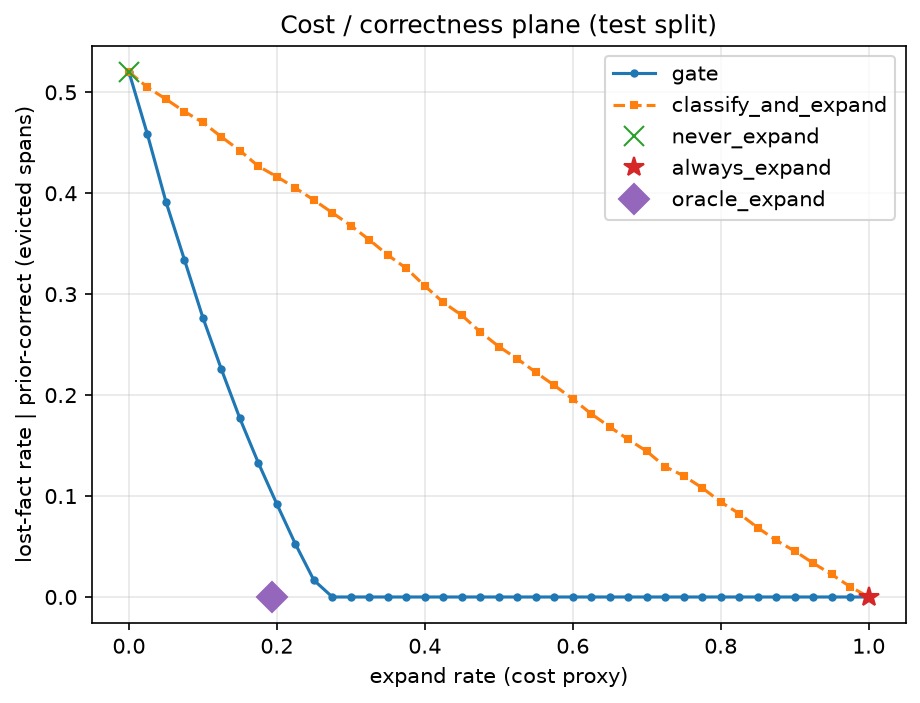
\includegraphics[width=0.72\linewidth]{figures/cost-correctness-plane.png}
\caption{Cost--correctness plane (test split). The gate curve dominates
query-type routing everywhere; oracle at $(0.194, 0)$; never-expand at
$(0, 0.52)$ pooled.}
\label{fig:plane}
\end{figure}

\begin{figure}[t]
\centering
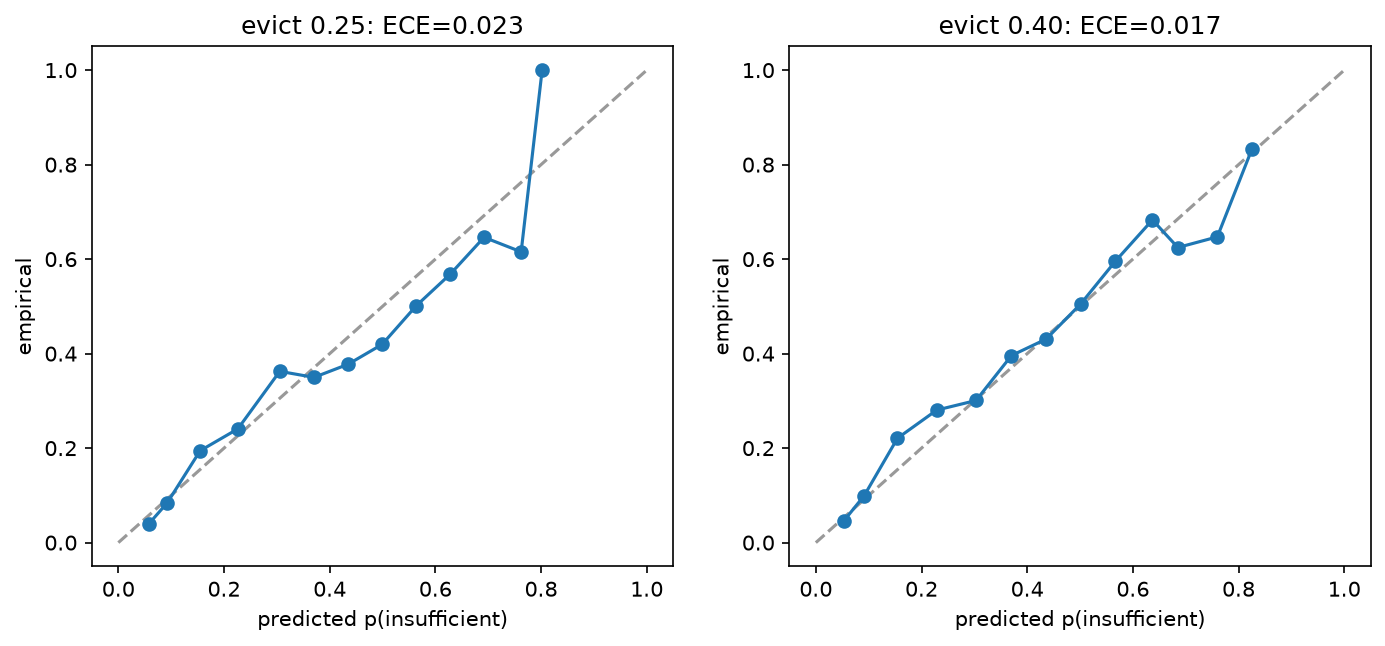
\includegraphics[width=0.85\linewidth]{figures/reliability-curves.png}
\caption{Reliability curves per eviction fraction; the linear probe is
natively calibrated ($T{=}1.0$; ECE $0.023$/$0.017$).}
\label{fig:reliability}
\end{figure}

\subsection{Multi-hop: the weakness moves to the cost axis}

On a 500-item slice of teacher-filtered two-fact questions composed within
single documents, the gate at the single-hop threshold \emph{holds
correctness}---\lostfact{} $0.036$ vs.\ $0.376$ never-expand---but does so
by over-expanding: recall $0.904$ at precision $0.388$, expansion rate
$0.438$ against an oracle of $0.188$ ($2.3\times$). The predicted
mid-spectrum weakness of retrieval-then-integration queries is real, but it
lands on cost, not correctness: a calibrated single-hop gate defends
multi-hop questions by firing too often. This cleanly scopes the next
component---a selector that scores block \emph{sets} so a multi-hop query
triggers one grouped expansion---and gives it a quantitative target
(recover ${\sim}2.3\times \rightarrow {\sim}1\times$ oracle cost at held
recall).

\subsection{Calibration does not transfer; discrimination does}
\label{sec:lodo}

Under leave-one-domain-out evaluation the gate's discrimination holds
(pooled AUC $0.781$--$0.865$; near-zero \lostfact{} at ${\approx}0.26$
expansion), but calibration degrades to ECE $0.05$--$0.13$. Fitting on
${\sim}200$ labeled items from the new domain repairs it---with a caveat
the ablation surfaced: a scalar temperature alone left three of four
domains above the $0.05$ bar ($0.071$--$0.073$); the cross-domain
miscalibration has a location component, and escalating to Platt scaling
(temperature $+$ bias on frozen scores) restores ECE to $0.014$--$0.035$
in every rotation (Table~\ref{tab:lodo}). The practical statement: a
``calibrated gate'' is not a checkpoint but a checkpoint plus a per-domain
recalibration procedure, and deployment to a new domain carries a small,
explicit labeling cost.

\begin{table}[t]
\centering
\caption{Leave-one-domain-out recalibration on ${\sim}200$ items from the
held-out domain (frozen gate scores).}
\label{tab:lodo}
\begin{tabular}{llcc}
\toprule
Held-out domain & method & ECE before & ECE after \\
\midrule
financial & Platt & $0.130$ & $0.014$ \\
legal & Platt & $0.106$ & $0.029$ \\
code & temperature & $0.064$ & $0.035$ \\
literature & Platt & $0.116$ & $0.023$ \\
\bottomrule
\end{tabular}
\end{table}

\section{The synthesis regime: a trained amortized compactor}
\label{sec:compactor}

The preceding sections certify \emph{untrained} eviction. We next train a
Still-class amortized compactor---one Perceiver per transformer layer
(per-KV-head latent banks, $d_l{=}256$, two pre-norm blocks with QK-normed
cross-attention at logit scale $d_l$, no FFN, ${\approx}50$M parameters),
with the RoPE-fix (keys inverse-rotated to a position-free frame,
compactor-internal RoPE at base 10, compact keys re-rotated at evenly
spaced output positions)---against the frozen base, and certify it under
the identical protocol. Two sanity gates precede training: an
identity-initialization pass-through test (with one latent per position,
compact-cache logits must match full-cache logits \emph{before} training;
this is the cheap detector for the position-metadata failure class) and a
loss-sanity bar (forward KL on rationale-trace answer tokens, top-200
teacher support, must fall below $0.4$ within 300 steps). Both passed.
Training used ${\approx}25$k teacher-rationale triplets at 8k context for
1{,}500 steps at effective batch 32---about $1/40$ of the published
recipe's data volume---so the certification below judges \emph{our
checkpoint}, not the method's ceiling.

\begin{table}[t]
\centering
\caption{Trained synthesis vs.\ untrained eviction at matched retained
budget (sinks + $t{=}1024$ latents + 1{,}024 recent raw slots of a
4{,}096-token context; 12 contexts across 4 domains). All rows on the
CERTIFICATION protocol (needle-anchored contexts); do not compare against
labeling-protocol numbers --- see Appendix~\ref{app:reconciliation}.}
\label{tab:compactor}
\begin{tabular}{lccc}
\toprule
arm & mean KL & acc.\ delta & lost-fact $\mid$ prior-correct \\
\midrule
control (no compression) & $0.000$ & $0.000$ & $0.000$ \\
eviction @ matched budget & $\mathbf{0.122}$ & $-0.049$ & $0.583$ \\
compactor, depth 1 & $0.263$ & $-0.090$ & $\mathbf{0.271}$ \\
compactor, depth 4 (recurrence) & $2.292$ & $-0.056$ & $0.750$ \\
\bottomrule
\end{tabular}
\end{table}

\paragraph{No-ship on the aggregation axis; a surprise on the pointwise
axis.} Table~\ref{tab:compactor}: at matched budget our compactor is
\emph{worse} than eviction on the aggregation axis (KL $0.263$ vs
$0.122$), so under our own deployment rule it does not replace eviction as
the default compressed tier. But the pointwise axis inverts: synthesis
\emph{halves} silent needle loss ($0.271$ vs $0.583$)---compact latents
are lossy blends that still carry needle content eviction deletes
outright. Both numbers sit far above the $0.000$ floor, so the
gate-mandatory rule re-attaches under every compaction regime measured.
The two compression families fail \emph{differently}, which strengthens
the case for certifying both axes rather than ranking compressors on
either alone.

\paragraph{Recurrence collapses.} Certifying at deployment recurrence
depth (re-compacting accumulated state chunk by chunk), depth 4 degrades
KL by $9\times$ (2.29) with $0.75$ needle loss---consistent with the
depth-validity envelope reported for Still-class compactors. We emit
\texttt{max\_certified\_depth}${}={}0$ into the compaction policy version
(weights hash included), and resume paths refuse to stack compactions past
it.

\paragraph{Gate refresh under the synthesis policy.} A new compaction
policy is a new label distribution, so we relabel all 98{,}355 items under
the compactor (old prefix synthesized, recent quarter raw; positive rate
drops to $0.167$) and retrain the gate. All operating-point and baseline
numbers in this paragraph and \S\ref{sec:routability} are on the LABELING
protocol (randomized context placement; Appendix~\ref{app:reconciliation}
reconciles it against the certification protocol above). Refreshed gate:
lost-fact $0.146$ at expansion $0.147$, ECE $0.007$; never-expand $0.189$;
oracle $0.000$ at $0.170$. The signal decomposition of
\S\ref{sec:mechanism} \emph{inverts}: embeddings-only ($0.567 \pm 0.005$)
now beats features-only ($0.537 \pm 0.002$; full $0.554 \pm 0.003$) ---
there is no eviction window for mechanics features to read, content
becomes the better predictor, and both are weak. What these numbers mean
for the router is the subject of the next section.

\section{Routable and unroutable loss}
\label{sec:routability}

Define a configuration's \emph{routability} as the fraction of its silent
pointwise loss that a calibrated per-query gate removes at an expansion
budget no larger than the oracle's. The two compression regimes, evaluated
on the same 98{,}355 items, the same test split, and the same (labeling)
protocol, differ far more in routability than in headline loss:

\begin{table}[t]
\centering
\caption{The routability asymmetry (labeling protocol, test split).
``Reduction'' is the gate's marginal effect vs.\ never-expand under the
SAME policy; ``budget use'' is gate expansion over oracle expansion.}
\label{tab:routability}
\begin{tabular}{lcccccc}
\toprule
regime & never & gate @ $\tau$ & oracle & reduction & budget use &
evicted-only AUC \\
\midrule
eviction & $0.520$ & $0.146$ @ $0.168$ & $0$ @ $0.194$ & $\mathbf{72\%}$
& $0.87$ & $0.62$ (mechanics) \\
synthesis & $0.189$ & $0.146$ @ $0.147$ & $0$ @ $0.170$ & $\mathbf{22.5\%}$
& $0.86$ & $0.55$ (content) \\
\bottomrule
\end{tabular}
\end{table}

Table~\ref{tab:routability}: the two \emph{systems} land on the same
operating point ($0.146$), but the credit assignment is opposite. Under
eviction the gate does the protective work; under synthesis the compressor
does, and the gate---spending the same $86$--$87\%$ of the oracle
budget---recovers only a fifth of what remains. The explanation is causal,
not incidental. Eviction's loss is \emph{mechanically} determined: a fact
is lost iff its span overlapped the eviction window, a condition legible
from bookkeeping features alone---which is exactly what the signal
decomposition found (features-only $\approx$ full model). Synthesis's loss
is \emph{content}-determined: it depends on what the compactor's latents
failed to preserve, a per-fact property that neither bookkeeping features
(no window to read) nor frozen gloss embeddings (AUC $0.55$) capture. The
same gap appears a third time in the multi-hop experiment: set-scoring
grouped expansion (rank-then-cut at the largest marginal-score gap, plus a
trained joint re-scorer) reduces the multi-hop cost overhang only from
$2.33\times$ to $2.15$--$2.24\times$ oracle, because grouping cannot
manufacture per-block discrimination the underlying scores do not carry.

Three design consequences. First, compressor choice determines
gate-ability: a compressor that loses less can still yield a \emph{worse}
routed system if its residual loss is unroutable, so certification must
report loss and routability together---neither number alone ranks
compressors. Second, the popular intuition that better compression
obviates routing is backwards on our evidence: as the compressor improves,
the router's job gets \emph{harder} per remaining failure, and the
lossless raw path (expansion) remains the only mechanism with a
correctness guarantee. Third, the binding constraint everywhere we looked
--- the gate's discrimination ceiling under both regimes and the multi-hop
overhang --- is one measured quantity, content-aware sufficiency
estimation, which we leave as the decision layer's open problem.


\section{Limitations}

Single base model and scale (4B). Our trained-synthesis comparison
(\S\ref{sec:compactor}) uses $1/40$ of the published data recipe; the
no-ship verdict certifies our checkpoint and budget, not the method---a
full-recipe run could reverse the aggregation-axis ordering (though the
depth-collapse and needle findings match the published pattern and should
be robust). Extractive MCQ probes with a letter-match equivalence function
rather than open-ended generation; greedy decoding; per-item single-turn
contexts rather than multi-turn threads; multi-hop limited to $k{=}2$
within-document composition. The dead content
pathway of \S\ref{sec:mechanism} may be a gloss-quality artifact
(extractive chunk prefixes and question-only query encodings) rather than a
fundamental limit; probing that requires summary-grade glosses and is left
open. The two-axis protocol itself is compressor- and model-agnostic; the
specific numbers are not.

\section{Conclusion}

Single-number long-context evaluation is incoherent under compression: the
pointwise and aggregative axes are antagonistic, and at 1B-token scale
they split almost completely. But the deeper lesson of certifying both
major compression families under one protocol is that loss itself is not
one thing. Eviction produces large, \emph{routable} loss: mechanically
caused, predictable from bookkeeping features, and removable at $72\%$ by
a ${\approx}\$140$ calibrated probe that never reads content. Synthesis
produces smaller, largely \emph{unroutable} loss: content-caused,
invisible to the same signals, leaving the gate a $22.5\%$ marginal
effect at the same relative budget. A compressed-memory system therefore
owes its users two numbers per configuration --- how much it loses, and
how much of that loss its router can recover --- and the architectural
conclusion stands regardless of compressor: a lossy tier, a lossless raw
path, and a calibrated router between them, with the router's
discrimination --- content-aware sufficiency estimation --- as the single
measured open problem, and per-domain recalibration as a shipped
procedure rather than a remark. That is where we think a memory system's
decision layer ought to leave its next iteration.

\bibliographystyle{plainnat}
\bibliography{references}

\appendix

\section{Evaluation-protocol record}
\label{app:protocol}
Every certification report object embeds: (i) the item partition per
axis---pointwise = needle items whose source chunk lies in the (reference)
eviction window; aggregation = a disjoint same-document set, with the count
of aggregation items whose chunks fall outside the certification context
(they score ${\approx}$chance under both conditions and dilute, but cannot
bias, the paired delta); (ii) compacted-context contents (surviving KV
only; no summary text or auxiliary representation); (iii) expansion
disabled during certification probing; (iv) scoring by argmax over
answer-letter logits under greedy decoding, making letter-format failures
structurally impossible; (v) the KL window length. All arms (control,
per-fraction, matched-random) share one probe partition; identical
prior-correct counts across arms ($21/25$) verify it.

\section{Baseline reconciliation}
\label{app:reconciliation}
The earlier certification numbers ($0.708/0.808$ raw; $0.550/0.650$
conditioned) and this paper's canonical never-expand rows ($0.453/0.551$)
measure different protocols. (1) \emph{Context construction}: the earlier
pass certified 20 packed contexts whose eviction window was anchored on the
needle chunk (adversarial placement; whole chunk always evicted); the
canonical protocol uses per-item 4096-token contexts with hash-randomized
placement, so evicted rows include boundary items with partial ($>0.5$)
overlap. (2) \emph{Denominators}: the earlier raw rates include never-knew
items (measured floor $0.167$); canonical rows have raw-correct
${\approx}1$ by construction (generation-time filtering plus greedy
determinism), so no never-knew inflation. (3) \emph{Pooling}: the pooled
$0.520$ mixes both fractions. The paper uses only the canonical per-item
protocol; the earlier numbers remain in the certification artifacts flagged
as a different protocol.

The same reconciliation applies to the synthesis regime, where never-expand
has two values in the record: $0.271$ on the CERTIFICATION protocol
(Table~\ref{tab:compactor}: needle-anchored 4{,}096-token contexts,
needles guaranteed inside the compacted region, matched-budget arms) and
$0.189$ on the LABELING protocol (Table~\ref{tab:routability}:
hash-randomized context placement, partial chunk overlaps counted as
compacted-away at $>0.5$, recent-raw window present). The certification
protocol is adversarial by construction and upper-bounds the loss; the
labeling protocol reflects the marginal placement distribution and is the
one the gate is trained and operated on. Binding rule used throughout:
Table~\ref{tab:compactor} and all axis-certification claims quote the
certification protocol; all operating-point, baseline, and routability
claims (Table~\ref{tab:routability}) quote the labeling protocol; the two
are never mixed within one comparison.

\section{Decomposition, seeds, and uncertainty}
Table~\ref{tab:decomposition} gives the three-variant decomposition
(3 seeds each). GT9-class headline metrics across seeds: \lostfact{}
$0.126 \pm 0.014$, expansion rate $0.177 \pm 0.007$. Bootstrap over test
items (1{,}000 resamples): \lostfact{} $0.146\,[0.136, 0.156]$, expansion
rate $0.168\,[0.163, 0.173]$, evicted-only AUC $0.622\,[0.608, 0.636]$.

\section{Corpus and filter survival}
Four ungated sources (SEC 10-K filings; US court opinions; permissive-license
source code; Project Gutenberg literature), 40{,}000 documents of
$\geq{\sim}6$k tokens, ${\sim}927$M tokens total. Counterfactual filters
retain ${\approx}38\%$ of generated items; per-domain yields
25{,}000/24{,}790/23{,}563/25{,}002 (financial/legal/code/literature).
Legal-domain source text carries OCR noise, visible as the weakest
per-domain gate recall.

\section{Reproducibility}
Pinned environment (torch 2.7.1, transformers 4.55.2, safetensors 0.5.3);
a 14-field compatibility fingerprint (model, tokenizer, chat template,
RoPE config, attention implementation, KV layout, quantization, runtime,
policy versions, kernel numeric probe) is stored with every KV artifact and
validated all-or-nothing. Compute ledger: corpus ${\approx}\$500$; labels
${\approx}\$110$; gate training, evaluation, multi-hop slice, and ablations
${\approx}\$30$; trained-compactor experiment (rationale data prep,
GT-gated 8$\times$H100 training sweep with an iterative family,
certification, relabeling, gate refresh, set-scoring evaluation)
${\approx}\$715$. Gate and compactor checkpoints, calibration records
(including per-domain recalibration entries), compaction policy versions
(weights hash + certified depth), evaluation grids, and all per-item
predictions are stored as content-addressed artifacts.

\end{document}
